\section{Introduction}
\label{sec:Introduction}

With widespread use of social medias, such as blogging services or social
network services (SNS), today we have become able to publish information
on the Web more easily than previously.  Especially recently,
microblogging services have been recently growing explosively.

Microblogging services are a new type of services which have both
characteristics of blogging services and SNS.  In microblogging
services, users can post short messages more easily and rapidly than in
conventional blogging services or SNS.  Microblogging services are not
necessarily regarded as a medium for publishing useful information to
the public, and many microblog users post messages more casually than in
conventional blogging services or SNS.  Because of these characteristics
of microblogging services, a large number of messages are posted on
microblogging services every day, and the messages contain various types
of contents, from personal notes or life logs to useful information or
discussion on specific topics. Furthermore, among these various types of
messages, those describing the current situations of the users posting
the messages especially characterize microblogging services.  This type
of message is far more frequent than in conventional blogging services
or SNS, on this account, a large number of messages posted on
microblogging services include information on real-time events.

Among many microblogging services,
Twitter\footnote{\url{http://twitter.com/}} is especially growing
rapidly.  As of 2012 December, Twitter has over 200 million active users
in the world\cite{TwitterUsers}, and as of June, more than 400 million
messages are posted on it per day\cite{TweetsPerDay}.  In Twitter, users
can post short messages with at most 140 characters, which are called
tweets.  By this limitation, Twitter makes information publishing more
easily and rapidly than conventional blogging services or SNSs.  The
most distinctive feature of Twitter is its mechanism of
\emph{''follow''}.  In Twitter, if a user follow other users, all tweets
by these followee users are retrieved in real time, and are shown in a
list sorted in the reverse chronological order, as shown in
Figure~\ref{fig:twitter}.  This list is called the \emph{''timeline''}
of the follower users.  The mechanism of follow is more casual than
user-linking functions in ordinary SNS; it does not require the
permission by the followee, and does not necessarily imply reciprocal
relationship. Another important function in Twitter is the
\emph{''reply''} function, by which a user can post a message as a reply
to another user.  By using this function, users can use Twitter for
conversation, as in instant messaging services.

{\footnotesize
\begin{figure}[t]
\begin{center}
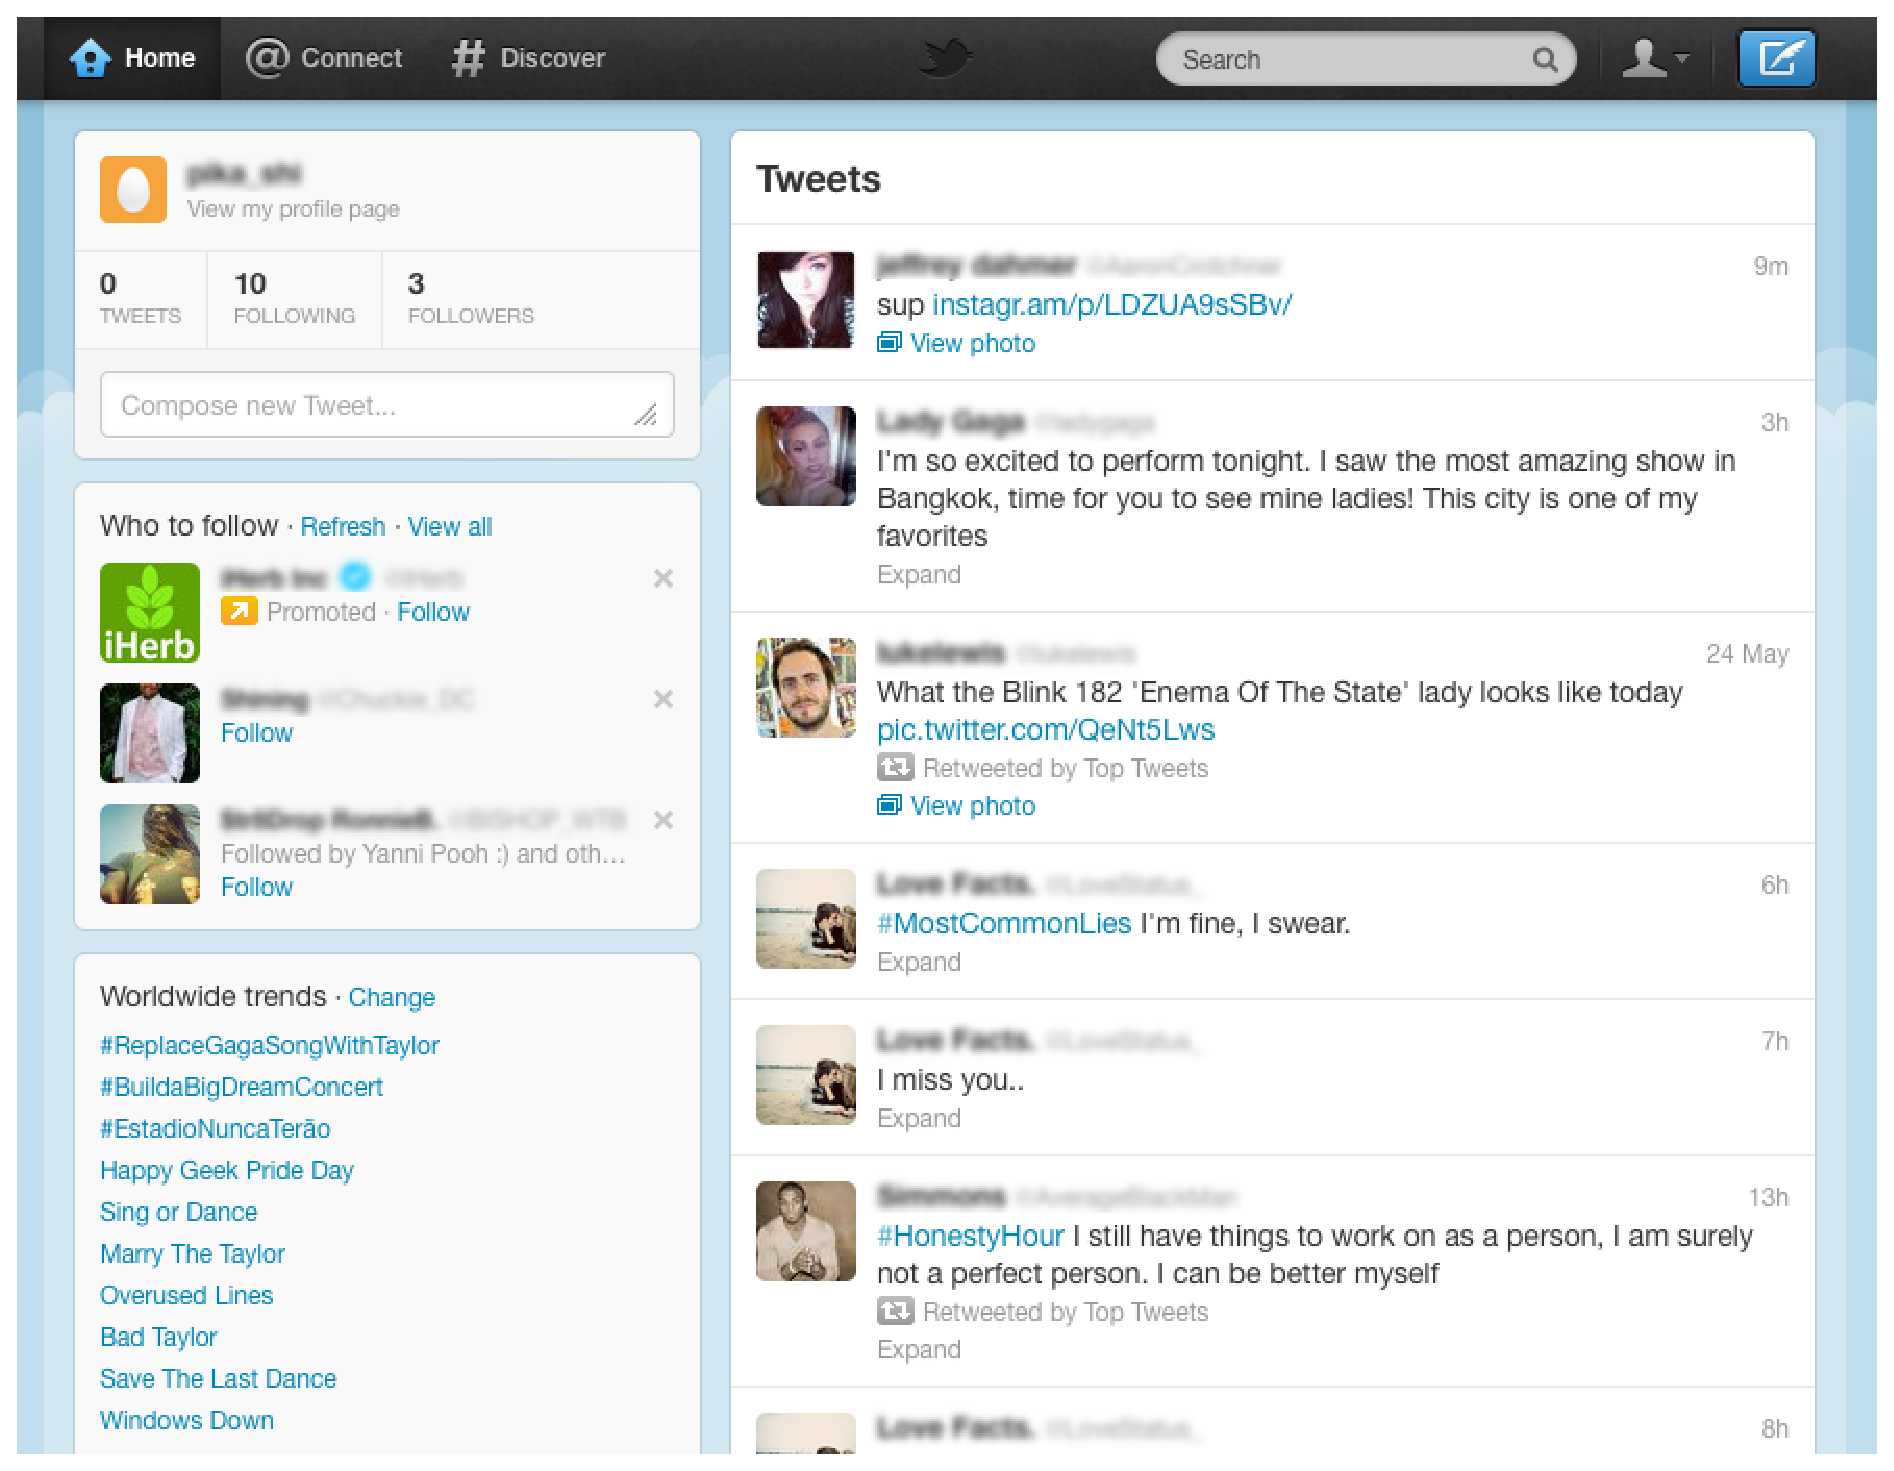
\includegraphics[width=14cm]{images/screen_shot.eps}
 \caption{An example of a user's timeline in Twitter}
\label{fig:twitter}
\end{center}
\end{figure}
}

Twitter has many characteristics of conventional social medias, and
because of this, it is used for many purposes.  Some users publish
information to the public widely like world news, some publish
information specified for certain topics, and some communicate with
their friends or others.  Because of this characteristic of Twitter, it
has attracted great attention as a new social media for information
publishing.

As explained above, Twitter is used for various purposes.  As a result,
the wideness of target scope of information publishing varies greatly
among users.  Therefore, in this study, we propose a method to classify
Twitter users from the point of view of how widely the target scope of
their information publishing is, i.e., whether they publish information
to the public widely or publish information specified in certain users.
In this study, we call the former \emph{``the target specificity is
low''}, the latter \emph{``the target specificity is high''}. In this
method, we focus on the followers of the user, and we classify him
whether his/her followers are consistent in some noticeable characters
or not.  If his/her followers are consistent in some noticeable
characters, it may be estimated that he/she publish information where
certain or particular users are interested. On the contrary, if his/her
followers are not consistent in any noticeable characters, there is high
probability that he/she is followed by a wide variety of users and it
may be estimated that he/she publish information where the public,
almost all users, is interested.

In addition, in this study, we focus on the Twitter user classified into
``the target specificity is high'' by the above method, and we propose a
method to determine what causes his/her target specificity, i.e., why
his/her target scope of information publishing is specified to certain
users.  In a large number of Twitter users, their target scopes of
information publishing are specified to certain users, and the causes of
their target specificities vary from user to user.  For example, a user
who publishes technical information about programming may suppose that
he/she publishes information toward unspecified users, but his/her
target specificity is considered high because the topic of his/her
publishing information is specialized to certain users who are
interested in programming.  And also, a user who communicates with
his/her friends or a user who announces to members of a certain club may
suppose that they publish information to the users specified
extensionally. So their target specificities are considered high,
regardless of contents of their publishing information.  In this method,
first, we roughly classify causes of the target specificity into two
categories: (1) because they publish information specified for certain
topics, and (2) because they publish information to the users specified
extensionally. And we construct a three-class classifier which determine
whether users only belong to category (1), only belong to category (2),
or belong to both category (1) and (2).  We then determine reasons that
the target specificity is high based on various features which
characterize each category for the classifier.  Figure~\ref{fig:Flow}
shows the overall flow of our methods.

{\footnotesize
\begin{figure}[t]
\begin{center}
\includegraphics[width=14cm]{images/flow.eps}
 \caption{Overall flow of our methods}
\label{fig:Flow}
\end{center}
\end{figure}
}

On the Web, it is hard to know what kinds of users each Web page targets
to.  But in Twitter, we can know what kinds of users each user targets
to by access to his/her follow relationships.  By exploiting this
relationships, we can estimate what kinds of users each user targets to,
thus we can classify users based on the target specificity of their
information publishing.

Twitter user classification of this study is considered to apply to
Twitter search.  In current Twitter search, we input a search in the
search box and receive messages including the keyword.  But with this
method, messages in search results has various target scope of
information publishing.  Thus, it frequency happens that messages of
certain target scope I need are buried in many other messages. For
example, when a user performs Twitter search with the word ``MacBook
Air'', what kinds of messages he/she needs depends on the situation of
that time, e.g., he/she may need public news about MacBook Air, he/she
may need technical knowledge about MacBook Air, or he/she may need
users' reviews of MacBook Air to refer when he/she buys new one.  But in
current Twitter search, these information is mixed up in search results.
At that time, by using Twitter user classification of this study, we can
search messages based on what kinds of users they target to.  In this
way, we can prevent messages users need from buried in many other
messages and help users to find messages they need easily.

The contribution of this paper is summarized as follows.

\begin{itemize}
\item We propose a new classification scheme of the target specificity
      of Twitter users' information publishing.
\item We show a method of classifying Twitter users based on above
      scheme.
\item As for users classified into ``the target specificity is high'',
      we show a method of determining the reason that the target
      specificity is high.
\end{itemize}

The rest of this paper is organized as follows.  Next section explains
some related work and makes the position of this study clear.  Then we
define Twitter user's target specificity of information publishing and
formulate our problem, and we discuss why target scope of some messages
in Twitter are confined to certain users in \ref{sec:Target
Specificity}.  In \ref{sec:ClassificationMethod1}, we explain the method
of classifying Twitter users based on how high the target specificity of
their information publishing.  In addition, in regards to Twitter users
classified into  ``the target specificity is high'' by the above method,
we explain the method of determining why their target specificities are
high in \ref{sec:ClassificationMethod2}.  Then in \ref{sec:Experiment},
we presents the results obtained from experiments we conducted to
evaluate the precision of our methods.  \ref{sec:Conclusion} concludes
the paper.

